	Infrared termography is a contactless way to measure infrared electromagnetic energy. It makes possible to observe contours of different bodies due to their temperature distribution, since every body is able to emit electromagnetic radiation when its temperature is above absolute zero. For this reason, it is a very important technology in military use, because it allows objects be seen even without proper illumination or in total lack of light situations.

	\begin{figure}[H]
		\centering
		\captionsetup{justification=centering}
		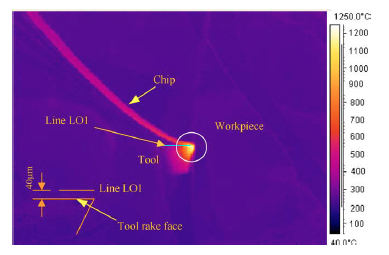
\includegraphics[scale=0.75]{Cap2/InfraRed/exinfrared.png}
		\caption{Infrared photography of a cutting process \cite{abukhshim2006heat}}
		\label{fig:exinfrared}
	\end{figure}

	The thermography tool is able to work in two different ways: passive and active. The passive way occurs when the subject matter has its temperature different from the environment (often higher). On the other hand, the active way needs an external heat source to induce a reasonable contrast between the object and the background \cite {maldague2000}.
	For the case under study, high speed thermography has its positive and negative points. On the positive side, it may be mentioned:
	\begin{itemize}
		\item Fast inspection rate (reasonable number of images of high speed cutting)
		\item Contactless (no interference during the cutting process)
		\item Easy interpretation of the results (indexed image with temperatures in each pixel)
	\end{itemize}
	But it is also important to mention the difficulties that in this method still prevail:
	\begin{itemize}
		\item Only a limited thickness can be measured (under the main surface)
		\item Determine a suitable emissivity is a chalenge (it changes with temperature variation)
	\end{itemize}